\chapter{Background}
\label{chap:backgnd}
\begin{abstractchap}
This chapter goes into detail about the notions of the theoretical our work is based on. First, we introduce the distributional hypothesis and the parameters involved in the generation of descriptive contexts from a corpus. Secondly, we present how can we describe the distributional contexts within a model, either directly through a vectorial representation or by means of a graph-based representation. Thirdly, we discuss one of the main challenges of dealing with textual data: data sparsity. We cover what is it, its consequences, as well as existent solutions to it. Finally, we summarize the concepts introduced and contextualize our propositions.
\end{abstractchap}
\minitoc

\section{Distributional Hypothesis}\label{sec:disto_hyp}
The work we present in this thesis is prominently based on the distributional hypothesis (DH). This is also the case for the large majority of semantic approaches in NLP today. This context-analysis insight is usually credited primarily to \cite{harris1954}. The hypothesis is simple yet powerful: it can be formulated as "You shall know a word by the company it keeps." \cite{firth57synopsis}. More formally, it states that the similarity of meaning correlates with the similarity of the word's context distribution. It follows that the meaning of a word can be determined by the set of contexts in which it occurs in a corpus. Consequently, for two target words, the larger the number of shared contexts, the semantically closer these words are. 

\begin{figure}
\centering
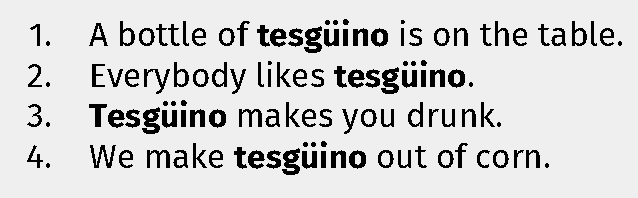
\includegraphics[width=.6\linewidth]{images/Chapitre2/tejuino.pdf}
\caption{Even though \textit{tesg\"{u}ino} is a relatively obscure word, from its context we can understand its an alcoholic drink made from corn.}
\label{fig:tejuino}
\end{figure}


Taking the classic example by \cite{nida1979componential}, shown in the four lines  in Figure \ref{fig:tejuino}, even if we do not know that the word tesg\"{u}ino (or tejuino) rinedefers to a ceremonial corn beer consumed by the native people of the north of Mexico, we can infer, by looking at its context, that we are indeed referring to some sort of corn alcoholic beverage. We can then easily infer that tesg\"{u}ino is similar to other drinks such as tequila or mezcal.



Although we usually find in the literature that the work of Harris is the most important concerning the DH, we should note that the hypothesis rests on two theories  \cite{sahlgren2008distributional,turney2010}: the statistical semantics hypothesis \cite{booth1955machine}, and the  structuralism theory, as described by \cite{de1916course}. The former is important as it places the DH within a larger context. Broadly, it affirms that statistical patterns of human word usage can be employed to understand what people mean. The latter,  gives the DH a more robust approach towards the definition of what kind of distributional context  we should use to determine similarities, as well as what does the meaning of the contextual relations between words implies. In plain words Saussure's version of the structuralist theory indicates that the differences in the contexts of a word determine its role within a language system. 

To this end, Saussure proposed two kinds of context relations: syntagmatic and paradigmatic. Syntagmatic relations concern the context defined by words that co-occur in the text, such as collocations (multi-word expressions that occur frequently in a corpus) and colligations (relations between a lexical item and a grammatical category) \cite{verschueren2015handbook}. On the other hand, paradigmatic relations associate words according to whether they appear or not in the same context. Put differently, these are words that tend to not appear together while sharing the same context. These type of relations define classic semantic relations such as synonymy-antonymy or hypernymy-hiponymy. Coupling both the DH with structuralist theory gives birth to the more fine-grained definition of the distributional hypothesis, introduced by \cite{sahlgren2008distributional}: the refined distributional hypothesis. We note that this distinction, syntagmatic versus paradigmatic relations, is also more recently defined in \cite{schutze1993vector}. In their work, syntagmatic relations are called first-order co-occurrences, while paradigmatic relations  are referred to as second-order co-occurrences.

\begin{figure}
\centering
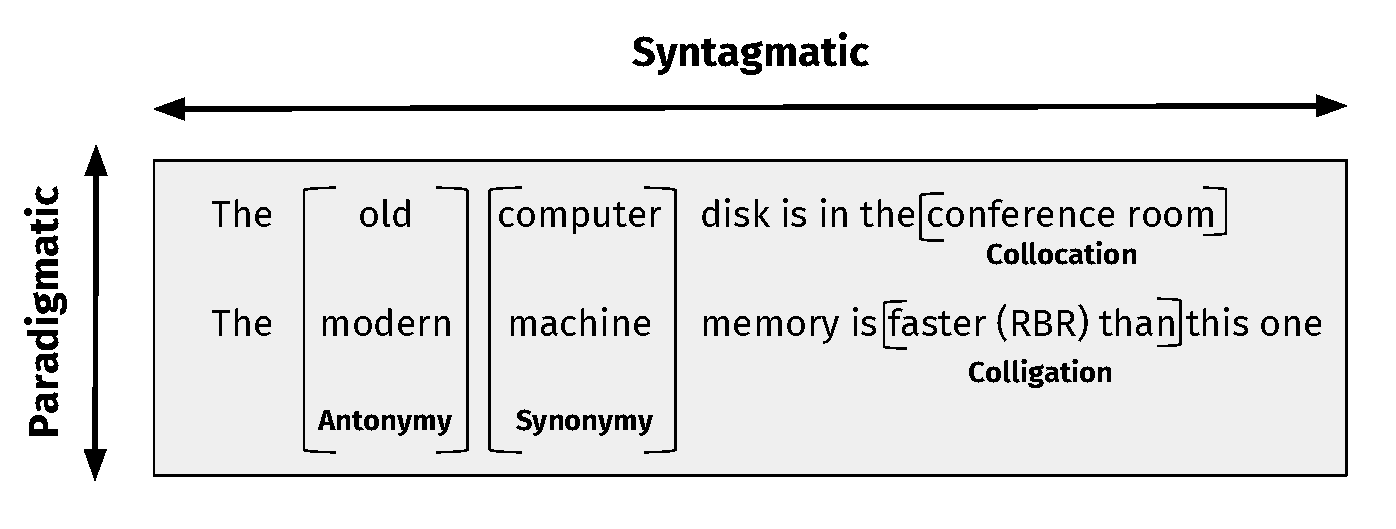
\includegraphics[width=\linewidth]{images/Chapitre2/sintagmatic_paradigmatic.pdf}
\caption{Examples of syntagmatic and paradigmatic contexts and their corresponding semantic relationships. Based on the examples by \cite{sahlgren2008distributional,piero2017}.}
\label{fig:sintagmatic_paradigmatic}
\end{figure}


An example of syntagmatic and paradigmatic relationships can be seen in Figure \ref{fig:sintagmatic_paradigmatic}. Vertically looking at the words \textit{old} and \textit{modern} (in the first and second phrase respectively), we can say that they  share a paradigmatic context, as they tend to not occur together, either we write old \textit{or} modern, while sharing the same context (either \textit{computer} or \textit{machine}). In this case, that leads to an antonym semantic relation. Something similar happens with the words \textit{computer} and \textit{machine}, this time sharing a synonym relation. With respect to the syntagmatic relationships, horizontally looking at the words, we find the collocation \textit{conference room} in the first phrase, as well as the colligation in the second expression between the word \textit{than} usually preceded by a  comparative adverb (RBR), which is \textit{faster} in this case. 

In spite of Sahlgren's  distributional hypothesis definition, determining the types and meaning of semantic relations, obtained with distributional methods, is still an open challenge on distributional models and methods. Determining the specific type of semantic relation (e.g., synonymy, hyponymy, meronymy) is still an open issue in the community \cite{turney2010,fabre2015,perinet2015}. While distributional models can give us fast access  to semantic relations between words within a corpus, they are most of the times ambiguous relations. It is still our task, as users, to determine the type of semantic relations found, in the case these distinctions are needed by the NLP system  at hand.
% We note that our work does not delves into the study of the semantic relations but we use them to relate 

Distributional methods, based on the DH, have been used for a long time now \cite{JurafskyM09}, although computationally automatized since the 1990s \cite{perinet2015}. Being a mature research field, systems based on these distributional models are varied and cover a large range of NLP tasks being obviously most popular on semantic tasks \cite{bruni2014multimodal}. We do note that nowadays, they have somewhat resurfaced (although they really never went away) thanks to the recent re-introduction of word embeddings, or simply word distributional representations. In short, a word embedding, in the context of newer developments, is a vectorial representation  that "embeds" words into a low-dimensional space, usually generated either by means of some sort of matrix reduction \cite{lebret2013deep,levy2014neural} or by using neural networks \cite{Collobert2011,mikolov2013distributed}. These representations are usually obtained from very large bodies of text and they have shown to be quite effective for solving NLP tasks.

The actual implementation of a distributional model consists in three steps: (1) determine what type of context is going to be used, (2) chose a computable context representation, and (3) determine a weighting scheme  and a  relatedness measure.

%\subsection{Types of Context}\label{sec:contexts}
We move now onto the description of what are the types of contexts commonly used while implementing a distributional model to represent words.  We cover two types: lexical co-occurrence and syntactic co-occurrence. In this work we will exclusively focus on those two contexts. The first one describes a word's context based on its nearby words.  The second defines a word's context according to the syntactic relations between the word and its neighbors. We will use the example phrases in Figure \ref{fig:example_phrases} to illustrate the kind of contexts we will describe below. 
\begin{figure}
\centering
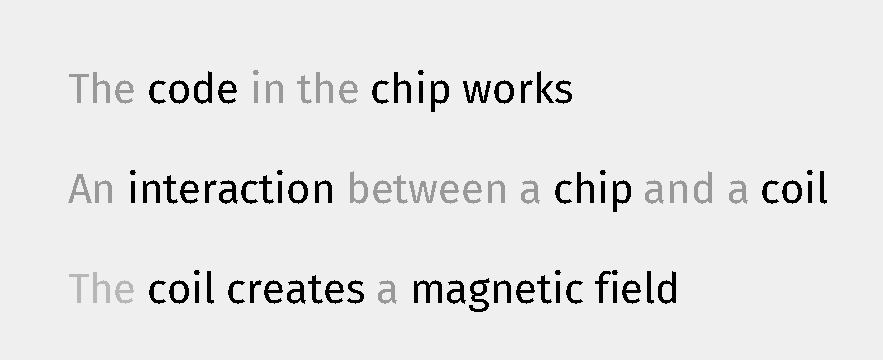
\includegraphics[width=0.7\linewidth]{images/Chapitre2/example_phrases.pdf}
\caption{Example text. Functional words are grayed-out. }
\label{fig:example_phrases}
\end{figure}

%todo Add as footnote the distinction between similarity and relatedness in Turney, Jurafsky, et al
%todo Define what is a target word (first time i talk about target word??)
%todo Add that a "Topical semantic relatedness" is obtained when context window is larger


\subsection{Lexical Contexts}
Also called linear contexts, lexical contexts consist on those  words that co-occur with a given word in a predetermined neighborhood: either in a sentence, a paragraph or larger units of text such as full documents \cite{LevyG14,sahlgren2008distributional}. Nowadays, the lexical context is usually determined by a window of $n$ tokens to each side of the target word. As an example is shown in Table \ref{tab:exo_lexical_contxt}, where the context -2+2 of the words \textit{code}, \textit{chip}, and \textit{coil} is shown. The size of the context depends of course of the application of the system. Indeed, determining the size  is actually a quite empirical decision. Nonetheless, it seems that today the literature \cite{Daume2006,mikolov2013distributed,LevyG14,levy2014neural}  has settled for a two-words to the left and two-words to the right context window (plus the target word), otherwise represented as -2+2. \cite{sahlgren2006word} discusses  the motivations of selecting a window of a particular size. He notes that given the literature evidence,  a shorter context window (specifically a -2+2 window) is preferable for acquiring semantic information. In this sense, \cite{JurafskyM09} determines that generally the context size used lies between 1 and 8 words on each side, or 3 and 17 in total. In practical terms, the choice of the size  affects the scope of the semantic relatedness: the shorter the context, the more specific is the information about a target word, approaching syntactic relations. Furthermore, these relations are "stronger" in the sense of being semantically similar, we could in theory substitute one word for another as the shared relation is synonymy. On the contrary, the larger the window, the broader the information conferred by the context words. 



% Please add the following required packages to your document preamble:
% \usepackage{booktabs}
\begin{table}[]
\centering
\caption{Lexical contexts of the words \textit{code}, \textit{chip}, and \textit{coil} appearing in each one of the phrases on Figure \ref{fig:example_phrases}. The context is paradigmatic, the window being the word and 2 words to the left and right.}
\label{tab:exo_lexical_contxt}
\begin{tabular}{@{}ll@{}}
\toprule
Words & Lexical Context                        \\ \midrule
code  & code;\textbf{w+1}:chip; \textbf{w+2}:works                    \\
chip  & \textbf{w-2}:interaction; chip; \textbf{w+1}:coil \\
coil  & coil;\textbf{w+1}:creates; \textbf{w+2}:magnetic              \\ \bottomrule
\end{tabular}
\end{table}

Lexical co-occurrences are the most popular way to represent distributional contexts. They are easy to obtain as there is no need for external information except the input corpus itself. 
 




%\subsection{Lexical Representations}
%\subsection{Syntactic Representations}
%
\subsection{Syntactic Contexts}

The second type of context depends on a more profound analysis of text. As its name implies, syntactic contexts are based on the analysis (or parsing) of text in order to obtain sense from them. Lexical contexts are able to somehow take into account the order of appearance of words in a phrase. Still, words in a sentence are not related among them like a list: semantic information is indeed extracted from words themselves, however syntax highly affects the way information is combined into semantic structures. Words tend to form groups between themselves, called constituents or chunks, which relate to other constituents to form a single phrase unit \cite{bender2013linguistic}.

\paragraph{Constituent Tree}
Indeed, constituents are  represented with tree structures aptly named  constituents parse tree, or simply parse tree (see Figure \ref{fig:exo1_constits}) \cite{JurafskyM09}. These trees actually represent the context-free grammars models that we use to describe the chunk structure. As such, the parse tree differentiates between terminal, pre-terminals and non-terminal nodes. Non-terminal nodes refer to chunk labels (e.g., noun phrases\footnote{The nomenclature used is the Penn Tree Bank annotation.}: \textit{NP}, verbal phrases: \textit{VP}, prepositional phrases: \textit{PP}), pre-terminal nodes pertain to Part of Speech (PoS) categories (e.g., determinants: \textit{DT}; adjectives: \textit{JJ}; nouns: \textit{NN}). Finally, terminal nodes indicate the word itself. 

%todo References, who is using constituents trees??
A constituents tree is illustrated in Figure \ref{fig:exo1_constits}. The image corresponds to the parse tree of the first phrase of the example in \ref{fig:example_phrases}: \textit{The code in the chip works}. From the bottom-up,  looking at the node labeled \textit{chip}, we see it is a token of type noun (pre-terminal labeled \textit{NN}) and it belongs to a noun phrase (non-terminal \textit{NP}) which in turn belongs to a prepositional phrase (\textit{PP}) which finally is part of the main noun phrase of the sentence \textit{S}. Constituents usually include a word with a prominent role: the \textbf{head} of the constituent. In practical terms, the head (or governor) is the most important word in the chunk because it determines what kind of words (either a verb, an adjective, a noun, etc.) will be joining it within the constituent. 

The context that can be extracted from a constituency parse is similar to that of the lexical contexts, in that words themselves are part of the co-occurrent neighborhood. Yet, with the information from the parse tree, we can restrict the window to a chunk and heal consider only certain structural units. The context of \textit{code} and \textit{chip} of the parse  in Figure \ref{fig:exo1_constits} are shown in Table \ref{tab:exo_constits_contxt}. They consist simply in the non-functional words that co-occur with each word in a given constituent, in this case a noun phrase (NP).

\begin{figure}[t!]
	\begin{minipage}{\textwidth}
		\begin{minipage}{.9\textwidth}
			\centering
			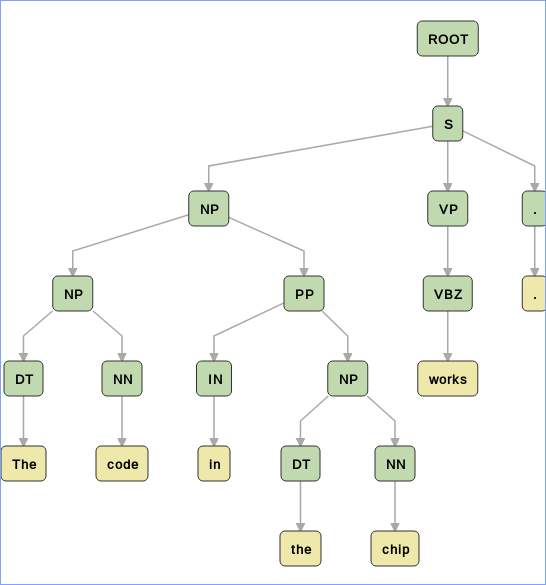
\includegraphics[width=0.7\linewidth]{images/Chapitre2/exo1_constits.png}
			\captionof{figure}{Constituents tree parse of the phrase \textit{The code in the chip works.}}
			\label{fig:exo1_constits}
		\end{minipage}
		\\
		\\
		\begin{minipage}{.9\textwidth}
			\centering
			\begin{tabular}{@{}ll@{}}
			\toprule
			Words & Syntactic Context                        \\ \midrule
			code  & \textbf{NP}:chip                    \\
			chip  & \textbf{NP}:code \\
			\end{tabular}
			\captionof{table}{Syntactic contexts, based on the constituents tree in Figure \ref{fig:exo1_constits}, corresponding to the words \textit{code} and \textit{chip}, from the first phrase on Figure \ref{fig:example_phrases}.} 
			\label{tab:exo_constits_contxt}
		\end{minipage}
	\end{minipage}
\end{figure}

%TODO What is a grammar?
\paragraph{Dependency Tree}
While  a parse tree represent the units existing within a specific group of syntactically related words, as a complementary approach, we can also formalize syntactic information with dependency trees. This time, the syntactic structure of a sentence is described in terms of words and asymmetric binary grammatical functions between these words   \cite{ClarkBook2010}. The trees are directed, all nodes are terminal and they represent words and they are linked following a direction from the head to its \textbf{modifier} (or dependent). An edge thus represent one of these dependency functions which are labeled  with tags that, just as PoS tags and chunk tags, describe what kind of relation exists between two words \cite{bird2006nltk}. For example, the Universal Dependencies\footnote{This set of tags share a large quantity of labels with the more classic Stanford Dependencies \cite{de2006generating,de2008stanford} tagset. Briefly, universal dependencies aim to develop cross-linguistically and cross-language consistent annotations  \cite{nivre2016universal}.} tagset \cite{nivre2016universal,schuster2016enhanced}, which we use in this work, includes tags such as  \textit{det}: determiner, the relation between a noun head (governor) and its determiner, \textit{nmod}: nominal modifier, the same but with a modifier, or \textit{conj}: conjunction, two elements connected by a conjunction.

To illustrate dependency trees, we can observe in Figure \ref{fig:exo1_dependences} the dependency parse of the second phrase shown in \ref{fig:example_phrases}. In this particular case, the relation tags used are the "enhanced" universal dependencies by \cite{schuster2016enhanced}. The difference is that relations are made more explicit by collapsing them (reducing two relation edges into a single one)  and including the modifier  (or adjunct) directly into the label. Consequently, they can be more useful to determine the relatedness between words.

The context that can be extracted from dependency relations varies. Still, the usual consensus is to treat the relation as the triple it is: $(head, relation, dependent)$ and based on it extract a certain type of context. In the example of Figure \ref{fig:exo1_dependences}, a context of the word  \textit{chip}, according to \cite{Lin1997} would be: $(conj:and,coil,head)$. This indicates that \textit{chip} is connected to \textit{coil} by the conjunction \textit{and}. More recent context definitions, such as those of \cite{baroni2010distributional,LevyG14,Panchenko2017} also include the inverse relation a word participates in, i.e., if the target word is a dependent, its dependency relation is also included but indicated as "inverse".  Again, using the previous example with the  word \textit{chip}, the  contexts now would then be: interaction/nmod:between$^{-1}$; coil/conj:and . These contexts and other example can be seen in Table \ref{tab:exo_deps_contxt}.

\begin{figure}[!t]
 \begin{minipage}{\textwidth}
  \begin{minipage}{.9\textwidth}
    \centering
	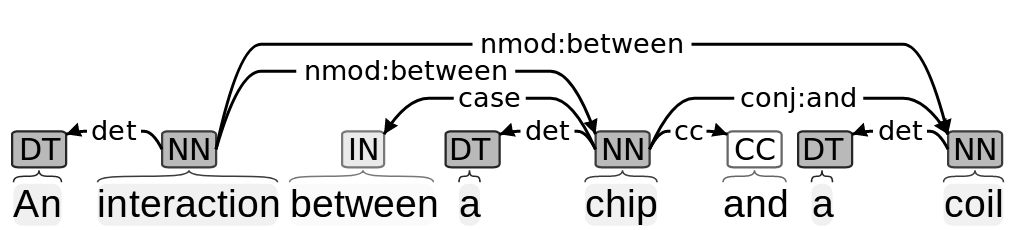
\includegraphics[width=0.9\linewidth]{images/Chapitre2/exo1_dependences.png}
    \captionof{figure}{Dependency tree parse of the phrase \textit{An interaction between a chip and a coil.}}
    \label{fig:exo1_dependences}
  \end{minipage}
  \\ 
  \\
  \begin{minipage}{.9\textwidth}
    \centering
		\begin{tabular}{@{}ll@{}}
		\toprule
		Words & Syntactic Context                        \\ \midrule
		interaction  &   coil/nmod:between; chip/nmod:between                   \\
		chip  & interaction/nmod:between$^{-1}$; coil/conj:and \\
		coil  & interaction/nmod:between$^{-1}$; chip/conj:and$^{-1}$      \\ \bottomrule
		\end{tabular}
		\captionof{table}{Syntactic contexts, based on the dependencies tree in Figure \ref{fig:exo1_dependences}, corresponding to the words \textit{interaction}, \textit{code}, and \textit{chip}, from the second phrase on Figure \ref{fig:example_phrases}} 
		\label{tab:exo_deps_contxt}
    \end{minipage}
  \end{minipage}
\end{figure}

Syntactic contexts are less used than their lexical counterpart in large part due to the process of obtaining the trees discussed before. While nowadays there are several software solutions able to extract this kind of information, the process is decidedly more complex than counting words in a lexical context setting. Furthermore, the information is not 100 \% accurate, as the systems are trained using human annotated banks of trees (called treebanks) which is in itself an ambiguous and hard process \cite{JurafskyM09,perinet2015}.  This difficulty stems yet another problem with syntactic information: syntactic parsers are not easily available for languages other than English and the rest of those in  the indo-european family. As a last downside, these contexts are known to generate sparse computational representations as they are more specific than simpler lexical contexts \cite{sahlgren2006word}. Still, syntactic contexts are shown to be able to contribute more information about word's relations than simple lexical contexts \cite{Lin1997,pado2003constructing,turney2010,baroni2010distributional,LevyG14,Panchenko2017}. In other instances, lexical contexts are shown to perform better in NLP tasks except when the syntactic contexts are extracted from very large corpora (such as Google Syntactic N-gram corpus \cite{goldberg2013dataset} containing $10^{11}$ tokens) \cite{kiela2014systematic}.

We have presented the two  main types of co-occurrence contexts that can represent a word in a corpus. In the next section we present the structures that allow mathematical and computational manipulation of the information provided by these contexts.







%\blindtext %1 %7 lineas x 8.3 =~ 60 lineas


\section{Vector Space Models}

The whole point of determining contexts, either lexical or syntactic, for a set of words in a corpus is to be able to assess how similar their meaning is among them. This assessment of relatedness thus need to be measured by a metric in order to determine its level. The way we measure the relatedness between words relies on well-known algebraic operations, such as the dot  product. In order to calculate a dot product we need vectors. It follows that to calculate relatedness among words we need to represent words by means of vectors, where each vector describe a word and each dimension a context of it. 

The Vector Space Model (VSM) consists in representing textual units in a multi-dimensional space. The textual units represented are not constrained to words themselves. We may describe co-occurrent features for documents, phrases, paragraphs, or other types \cite{manning1999foundations}. A matrix is used as the structure that holds each object and its context features. Indeed, in practical terms, a VSM is then an array of real-number vectors, where each one represent a text unit and the columns describes the co-occurrent contexts the word participates in. To illustrate  this, in Table \ref{tab:lexical_matrix} we represent words of the previous examples in a \textit{word space}. Each entry of this matrix (called a co-occurrence matrix) represent a weight that infers the importance of the row word (or target word) with respect to the column (context) co-occurrence in a given context, within an input corpus \cite{JurafskyM09}. That is, the word \textit{code}, co-occurs once with the context indicated by the second and third columns, which in turn correspond to the words \textit{chip} and \textit{works}.
%We note that some vector space models are not constrained to 2-dimensional matrices and leverage structures of larger dimensions \cite{baroni2010distributional}.

In the example, the weights consist merely on the frequency of co-occurrence of each word with each context. Indeed, there are still other two related parameters that affect the meaning extracted from a distributional model: the weight each cell in the matrix has, or how do each co-occurrence affect each word; and the similarity measure  between vectors we will use to determine the semantic relatedness among words. For a complete analysis on a wide range of parameters affecting vector space models, see \cite{baroni2010distributional,kiela2014systematic,levy2015improving}.



\begin{table}[]
\centering
\caption{Matrix representation of the lexical contexts of the words appearing in the phrases of Figure \ref{fig:example_phrases}. The window is the complete phrase where the word occurs.}
\label{tab:lexical_matrix}
\begin{tabular}{@{}lrrrrrrrr@{}}
\toprule
 Words & \multicolumn{8}{c}{Contexts} \\ \midrule
       & $w_1$ & $w_2$ & $w_3$ & $w_4$ & $w_5$ & $w_6$ & $w_7$ & $w_8$ \\ \midrule
code$_{w_1}$        & 0    & 1    & 1     & 0           & 0    & 0       & 0        & 0     \\
chip$_{w_2}$        & 1    & 0    & 1     & 1           & 1    & 0       & 0        & 0     \\
works$_{w_3}$       & 1    & 1    & 0     & 0           & 0    & 0       & 0        & 0     \\
interaction$_{w_4}$ & 0    & 1    & 0     & 0           & 1    & 0       & 0        & 0     \\
coil$_{w_5}$        & 0    & 1    & 0     & 1           & 0    & 1       & 1        & 1     \\
creates$_{w_6}$     & 0    & 0    & 0     & 0           & 1    & 1       & 1        & 1     \\
magnetic$_{w_7}$    & 0    & 0    & 0     & 0           & 1    & 1       & 0        & 1     \\
field$_{w_8}$       & 0    & 0    & 0     & 0           & 1    & 1       & 1        & 0     \\ \bottomrule
\end{tabular}
\end{table}

%todo slides the word-embeddings.pdf page 34 would be cool to put in this chap
%1 weighting
\subsection{Matrix Weights}

The weight is an important parameter in the creation of a VSM for a NLP application. Weights can be binary, simply  indicating presence or absence. They can count the number of co-occurrences of a word and the context, their absolute frequency. Weights may also be a type of discriminative measure that usually tries to give more importance to those contexts that co-occur more frequently with the target word while being less frequent  with the rest of the words in the text \cite{JurafskyM09,ClarkBook2010}.  

Point-wise Mutual Information (PMI) \cite{Church1990} and Positive Point-wise Mutual Information (PPMI) \cite{niwa1994co} are two popular choices to weight terms in a co-occurrence matrix \cite{turney2010,JurafskyM17}. We describe both of them below.

Given a co-occurrence matrix M, containing $W$ words (rows) and $C$ contexts (columns), where $f_{ij} \in \mathbb{R}^{W\times C}$ denotes the frequency of  target word $w_i$ frequency in the context $c_j$ , i.e., how many times they both co-occur. $N=\sum_{i=1}^W\sum_{j=1}^Cf_{ij}$ represents the sum of all the matrix cells. PMI is defined as:
\begin{equation} \label{eq:pmi}
PMI(w_i,c_j) = \log\dfrac{P(t_{ij}|c_j)}{P(t_{ij})P(c_j)}
\end{equation}
where  $P(t_{ij}|c_j)=\dfrac{f_{ij}}{N}$ tells us how many times the word and the context appeared together, normalized by the total context frequency. $P(t_{ij})= \dfrac{f_{ij}}{N}$, and $P(c_j)=\dfrac{f_j}{N}$. The ratio gives us an estimate of how much more the target and context co-occur than we expect by chance.

While PMI is often used as a weighting choice, it has three main downsides \cite{JurafskyM17,levy2015improving}: (1) PMI is biased towards co-occurrences of rare events, that is, a low-frequency context $c$ co-occurring with any word $w$ will yield a large PMI. Also (2), PMI may yield negative values, which would indicate a certain level of semantic "unrelatedness", which is not a  very intuitive concept. And (3),  if a context and a target word are not observed together (something that is very possible to happen because the co-occurrence matrix is sparse, we will look into that in the following paragraphs), the denominator of \ref{eq:pmi} is zero and thus $PMI_{ij}$ becomes undefined. 

To solve the first issue, \cite{levy2015improving} proposes a smoothed version of PMI, defined as:
\begin{equation} \label{eq:pmi_levy}
PMI_\alpha(w_i,c_j) = \log\dfrac{P(t_{ij}|c_j)}{P(t_{ij})P_\alpha(c_j)}
\end{equation}

with $P_\alpha(c_j) = \dfrac{f_j^\alpha}{N^\alpha}$, where $\alpha$ is a smoothing parameter that affects the contexts counts in order to alleviate the bias of PMI towards rare contexts co-occurrences : the probability of a low-frequency context $c_j$ will be larger thanks to $\alpha$, which makes the denominator of \ref{eq:pmi_levy} larger, which in turns make PMI$_\alpha$ smaller. Thus, addressing the bias for all words when co-occurring with a low-frequency context.


The second and third inconvenient are resolved by using Positive Point-wise Mutual Information (PPMI). PPMI simply replaces all values lower than zero (including $-\infty$) by a zero:
\begin{equation} \label{eq:ppmi}
PMI(w_i,c_j) = \max(PMI(w_i,c_j), 0)
\end{equation}
%2 similarity
\subsection{Defining Vector Similarity}
%3 sparsity (long, important paragraph)
The second parameter to consider after weighting the co-occurrence matrix is how to actually determine the similarity between two word vectors.

As with weighting schemes, there are multiple metrics (defined and compared to greater detail in \cite{ClarkBook2010,ferret2010testing,kiela2014systematic,clark2015vector}) used in the literature to determine the similarity between two vectors. We will focus on two that are of interest to this thesis: cosine and Jaccard similarity. More types of metrics and their comparison can be found in the previously cited literature. While there does not seem to be a single best measure of similarity, we usually use the cosine similarity, as it naturally can deal with real-valued vectors. On the other hand, when dealing with binary presence-absence vectors, it is more common to use Jaccard similarity. 

\subparagraph{Cosine Similarity}
The cosine similarity determines the angle between two multidimensional vectors. It is simply defined as the dot product between two vectors, normalized by the multiplication of their Euclidean length \cite{Manning2008}. The cosine similarity is bounded between $[0,1]$, yet we usually interpret the result in the positive space, where 0 means there is an angle of $90^\circ$ between the two word vectors, thus  no similarity at all; and 1 means there is no angle between them, so they are completely similar. Furthermore, if the weights of the matrix are non-negative values, the cosine similarity is bounded to the range $[0,1]$. The cosine similarity is defined as:
\begin{equation}
sim_{cosine}(\overrightarrow{w_1},\overrightarrow{w_2})  =  \dfrac{\overrightarrow{w_1}  \cdot \overrightarrow{w_2}}{||\overrightarrow{w_1}||\,||\overrightarrow{w_2}||} = \dfrac{\sum_{i=1}^Cw_{1_i}\times w_{2_i} }{\sqrt{\sum^C_{i=1}w_{1_i}^2}\sqrt{\sum^C_{i=1}w_{2_i}^2}}
\end{equation}

\subparagraph{Jaccard Index}
Also known as the Tanimoto index, the Jaccard index \cite{jaccard1908nouvelles} determines the similarity between binary vectors, it is defined, in terms of dot products:

\begin{equation}
sim_{Jaccard}(\overrightarrow{w_1},\overrightarrow{w_2}) = \dfrac{\overrightarrow{w_1} \cdot \overrightarrow{w_2}}{||\overrightarrow{w_1}||^2+||\overrightarrow{w_2}||^2 - \overrightarrow{w_1}\cdot\overrightarrow{w_2}}
\vspace{1cm}
\end{equation}

In terms of two sets, $A$ and $B$, the Jaccard index  calculates the ratio between the cardinality of the intersection of two word vectors divided by the cardinality of their union: $sim_{	Jaccard}(A,B)=\dfrac{|A \cap B|}{|A \cup B|}$. We prefer the definition in terms of dot products because in that way it is more straight-forward to implement it computationally.

We have been discussing vectorial space representations and their parameters (matrix weighting, similarity measure). While VSM models are the most popular to describe the semantic similarity between words, there are other structures that make it easier to  model the interactions that take place among lexical units within a corpus. In that sense, in the next section we introduce the fundamentals of graph-based representations for NLP, which are part of the contributions of this thesis.


\section{Network Models}
Network\footnote{We will use the notion of \textit{network} and \textit{graph} interchangeably during the rest of this dissertation, unless stated otherwise.} based models have been studied deeply during the last years in the NLP field  \cite{Mihalcea2011}. While we can represent a graph as a matrix, and thus as a vector space model, graphs are useful representation formalism that can be applied to a large set of linguistic characteristics, from the relation between words in a text or between the features that describe them. Indeed, language being a dynamic complex system, networks provide an adequate model to represent and study the structure and evolution of linguistic systems \cite{Choudhury2009}. 

Furthermore, based on graph theory, we can conceive efficient and sophisticated solutions to NLP tasks, such as PoS tagging, role-labeling, word sense induction and disambiguation, chunk parsing \cite{Mihalcea2011}. Notably, NLP graph-based approaches are largely employed to solve unsupervised tasks, where we can expect to get insights from the data by looking at  the links existing between entities; and semi-supervised problems, again by leveraging relations to propagate across the network small quantities of hand-crafted tags \cite{nastase2015}. An additional non-negligible advantage of graph models are that they allow human interpretation and analysis through their visualization (nonetheless with relatively small samples of text). 


Based on the  advantages just mentioned, in this thesis we base our linguistic\footnote{We will refer to a linguistic representation as an structure that holds textual units linked by their linguistic features, in this case, distributional co-occurrences.} model proposition on a graph-based structure. In the following paragraphs we discuss the types of networks used to represent textual data, which closely relates to the co-occurrence representations that we covered in the vector space model. Indeed, graph-based methods follow the same distributional principles as VSM. Thus, as we will see, the relationships among nodes on these networks are very similar to the types of contexts described in Section \ref{sec:disto_hyp}.


\subsection{Linguistic Networks}
A graph is a data structure consisting of a set of vertices connected by
a set of edges that  model relationships between objects.
Formally it is defined as a set $G=(V,E)$, where $V$ is a
collection of vertices $V=\{V_i,i=1,n\}$ and $E$ is a collection of
edges over $V$, $E_{ij}=\{(V_i,V_j),V_i \in V, V_j \in V\}$. 

When referring to language networks, nodes represent lexical units (most of the time words) and the edges represent the relationships between words. We present below the types of linguistic networks. 

\subsection{Types of Linguistic Networks}

According to their objectives, we can consider two types of contributions in the linguistic-network literature: on the one hand, there are those approaches that investigate the nature of language via its graph representation, and on the other hand, we find those that propose a practical solution to a given NLP problem  \cite{Choudhury2009}. In particular, we pay attention to two aspects of a given network-based technique: (1) the  characteristics of the linguistic data within the network, and (2), the  algorithms used to extract knowledge from it.


In the following paragraphs we introduce the general categories of linguistic networks according to their type of content and relations. We will introduce these categories as well as the  approaches that make use of them.

\cite{Mihalcea2011} defines four types of Language Networks (LN): co-occurrence network, syntactic-dependency network, semantic network and similarity network. Meanwhile, from a deeper linguistic point of view, \cite{Choudhury2009} introduces broader network's categories, each having several sub-types. The main difference (in our context) between both definitions lies in the separation of categories. In \cite{Choudhury2009}, they conflate syntactic-dependency and co-occurrence networks into the same  category: word co-occurrence networks. Similarly, they join semantic and similarity networks together and place them inside a broader category of lexical networks. The third  family  defined concerns phonological networks which is out of the scope of this work. In this work we will explore four categories of linguistic networks: lexical co-occurrence, syntactic co-occurrence, semantic and heterogeneous networks. Based  on the previously cited works, the following paragraphs will elucidate what does each kind of network represent.
%These difference will be developed in subsection \ref{} and \ref{} where we discuss the nature of the language network graph as well as the algorithms used to obtain a practical solution to a NLP task.



\paragraph{Lexical Co-occurrence Networks (LCN)}
%An effective way to  represent word co-occurrences is by means of a graph structure. Indeed, this kind of graphs are the central column of a Lexical Co-occurrence Network.

 In these structures, nodes represent words and edges indicate co-occurrence between them, i.e., two words appear together in the same context. The context is also defined by a window of terms. It may vary from a couple of words to a full document, although it is usually defined at sentence level. The edges' weight  represent the strength of a link and is generally a frequency based metric that takes into account the  number of apparitions of each word independently and together. Thus, usually the same type of weights as described are used to represent the \textit{strength}  of a relation. An example of such network is shown in Figure \ref{fig:lex_net1}. The words such as \textit{control, systems, power} co-occur in the same window of terms to the word \textit{project}.

\begin{figure}[!h]
\centering
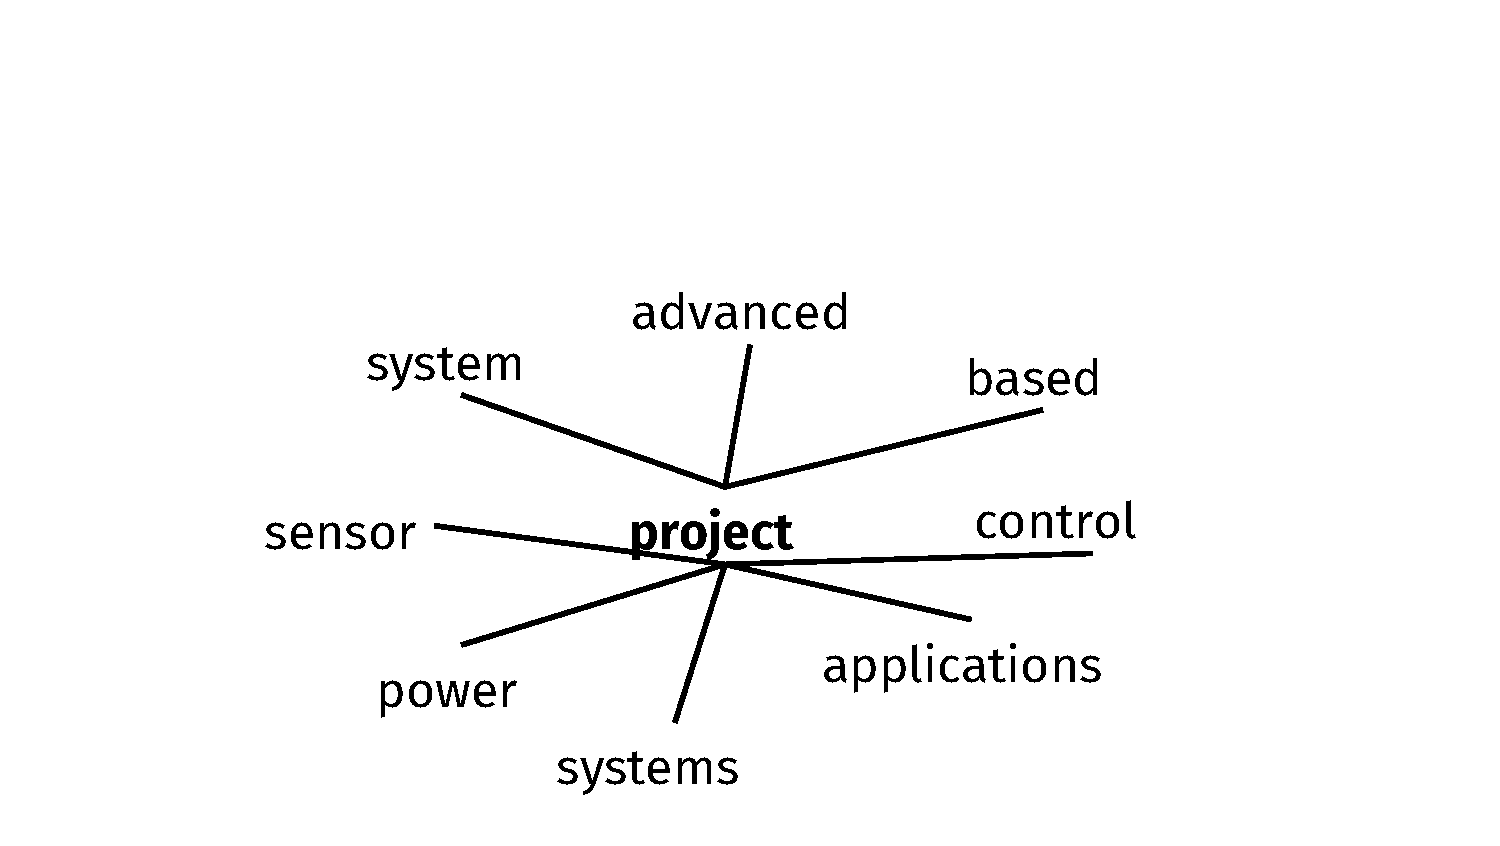
\includegraphics[width=0.8\linewidth]{images/Chapitre2/lex_net1.pdf}
\caption{Lexical network for the word \textit{project}.}
\label{fig:lex_net1}
\end{figure}


\paragraph{Syntactic Co-occurrence Networks (SCN)}
A Syntactic Co-occurrence Network (SCN) is very similar to a LCN  in the sense that both exploit the distributional hypothesis. Nonetheless, SCNs go further by leveraging  syntactic information extracted from the text. Both of the two types of syntactic parses are used: constituency-based  and dependency-based parse trees. SCNs employ, most of the time, dependency trees to create a graph that relates words according to their syntactic relations.  In Figure \ref{fig:syn_net1}, a small syntactic network is shown. In this case, the head word \textit{color} is related to the words \textit{sky} and \textit{weight} by means of a noun-modifier dependency relation  (\textit{nmod}). Other words are linked similarly according to other dependency relations.

%In the case of \cite{2013.Hope.GradedWSI}, a graph is built using syntactic dependencies.
 These networks are usually used to perform WSI employing a very similar approach to those systems using LCNs. As before, the main difference being the semantic relatedness found with one or another type of network.


\begin{figure}[!h]
\centering
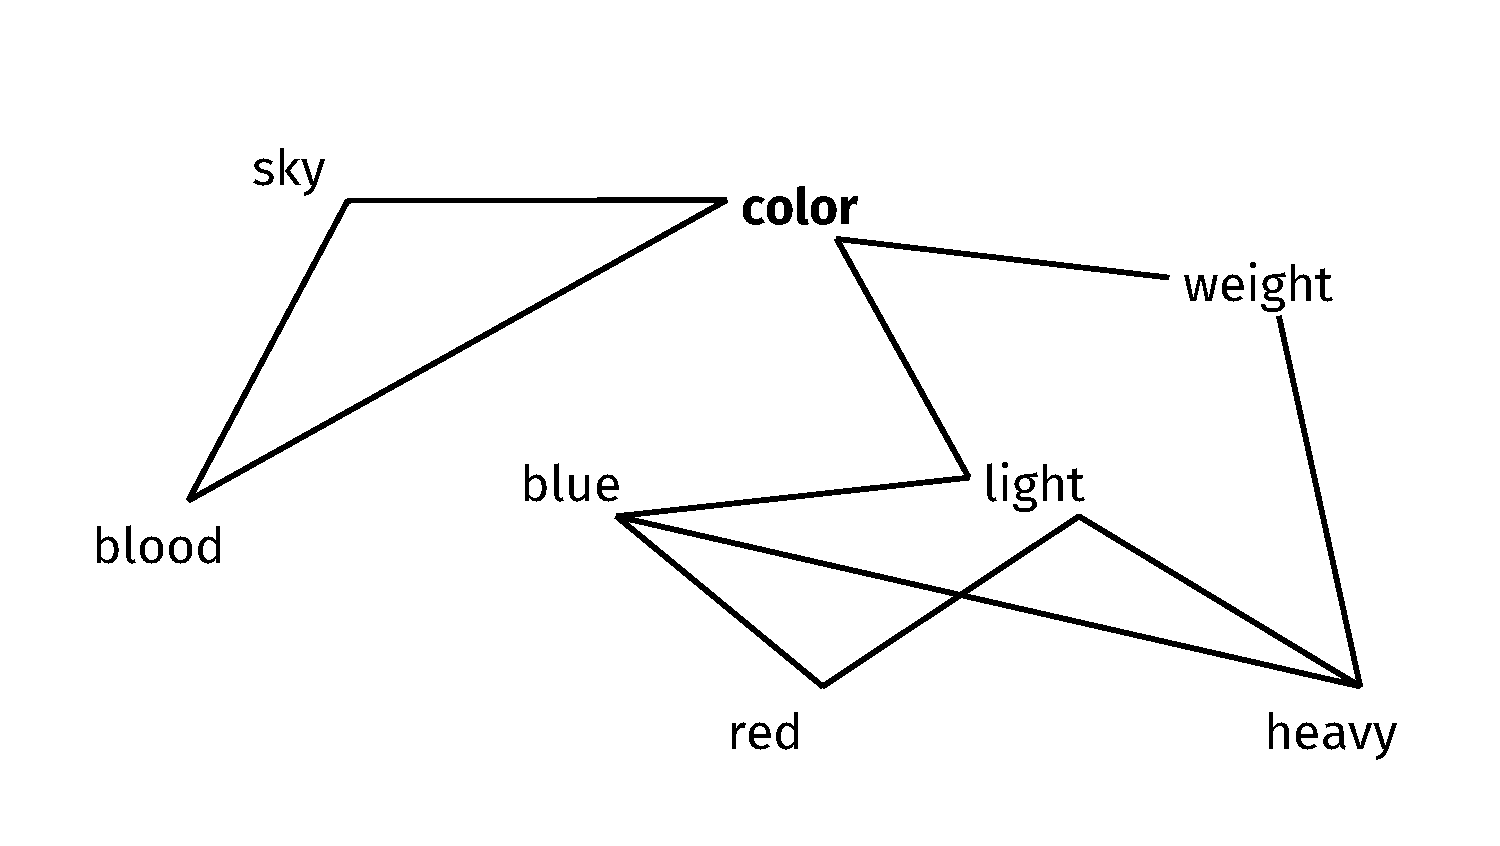
\includegraphics[width=0.7\linewidth]{images/Chapitre2/syn_net1.pdf}
\caption{Syntactic Network of the word \textit{color}.}
\label{fig:syn_net1}
\end{figure}

\paragraph{Semantic Networks}
A Semantic Network (SN) relates words, or concepts, according to well-defined semantic relations. The classical example of a SN is the renowned knowledge base Wordnet. This network, which serves also as an ontology, contains sets of synonyms (called \textit{synsets}) as vertices and semantic relations as their edges. Typical semantic relationships include synonymy-antonimy, hypernymy-hyponymy, holonymy-meronymy. However, other semantic similarities can be defined. The edges are usually not weighted, although in some cases certain graph similarity measures may be used.

\begin{figure}[!h]
\centering
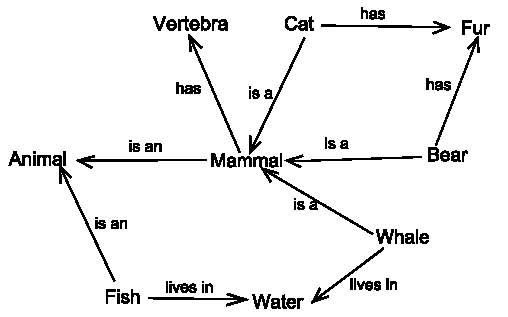
\includegraphics[width=0.7\linewidth]{images/Chapitre2/sem_net.pdf}
\caption{Semantic Network of the word \textit{mammal}.}
\label{fig:sem_net}
\end{figure}


\paragraph{Heterogeneous Networks}
Until now, we have described different types of networks with single types of nodes and relations. Lately, heterogeneous networks have been defined in order to model multi-typed information in a single structure \cite{Jiawei2009}. In reality, we could argue that syntactic-based and semantic networks are already heterogeneous on their own right, as both of them contain edges that represent different types of relations.



Without regards to their type, network-based structures are ultimately transformed into matrices before being treated computationally. Therefore, given that we are still modeling language (words), graphs suffer from sparsity just as vector space models. Indeed, data sparsity is an issue that affects the performance of knowledge discovery approaches \cite{mining12Book,PerinetH15} applied to textual data.

\section{Data Sparsity}
Representing word's contexts as multidimensional  vectors, either directly or through a graph-based structure, is indeed a straight-forward, simple and  yet powerful method to transform textual data into actionable structures. The model links  textual information, in the form of words and contexts, with the methods used in machine learning.

Nonetheless, there is an important issue that needs to be considered when dealing with vector space models: data sparsity.  A sparse data matrix has most of its entries equal to zero. Thus, the majority of the words (rows) in the corpus are described by very few contexts (columns). This is a significant problem as on the Knowledge Discovery phase of any NLP system we aim to train a learning model that will eventually predict, classify, group our words in one way ot another. If the words are represented by a limited number of context, the learning algorithms will not be able to generalize properly. Furthermore, when testing the systems, the system will not be able to handle unseen word-context co-occurrences. This will lead to reduced performance \cite{phan2008learning}.

This phenomenon is not the consequence of using vector space models per se,  as the vectors are merely a representation of  word's distribution within a text. Indeed, words tend to be distributed in a text in a very predictable fashion. In any natural language corpus, most of the words occur very few times. On the other hand, very few words occur multiple times. The consequence is that most of the entries in a co-occurrence are zero because we observe very few unique word-context co-occurrences. Put differently, words co-occur most of the times with the same words and  very few times with other words \cite{sahlgren2006word}. Given that any corpus is limited, acceptable English co-occurrences will be missing from it and their weight will be zero while they  actually happen in other corpora \cite{JurafskyM17}. To illustrate sparsity, Table \ref{tab:lexical_matrix} co-occurrence matrix contains eight words and eight contexts (each of the words), for a total of 64 entries. Among these entries, only 20 values are non-zero, and more importantly each word is only represented  by 2.5 contexts in average. While it is a toy example, and 20 non-zero entries from 64 in a matrix would hardly be considered sparse, it reflects what actually happens with larger corpora, as this problem is corpus-size independent (and even more important with smaller corpora \cite{perinet2015}). 

%\subsection{Dealing with data sparsity}
In order to deal with the distributional representation sparsity, we discuss below multiple techniques used in the literature \cite{sahlgren2006word,RatinovR09,piero2017} that aim to alleviate matrix sparsity.  In the following paragraphs we discuss explicit and implicit representations. We note that by explicit representation we refer to the classic weighted co-occurrence matrix, introduced before, where cell's values represent target word in a specific context. It is explicit in the sense that each column directly represent a context seen in the input corpus.
%


\paragraph{Implicit Representations}
These methods aim to reduce the sparsity as well as the dimension of the co-occurrence matrix while keeping latent (or implicit) features that best represent the original spaces. These techniques reduce the feature space to $k$ dimensions (usually $k$ is much smaller than the original number of columns) and thus the dimensions  are no longer directly interpretable.

\begin{figure}
\centering
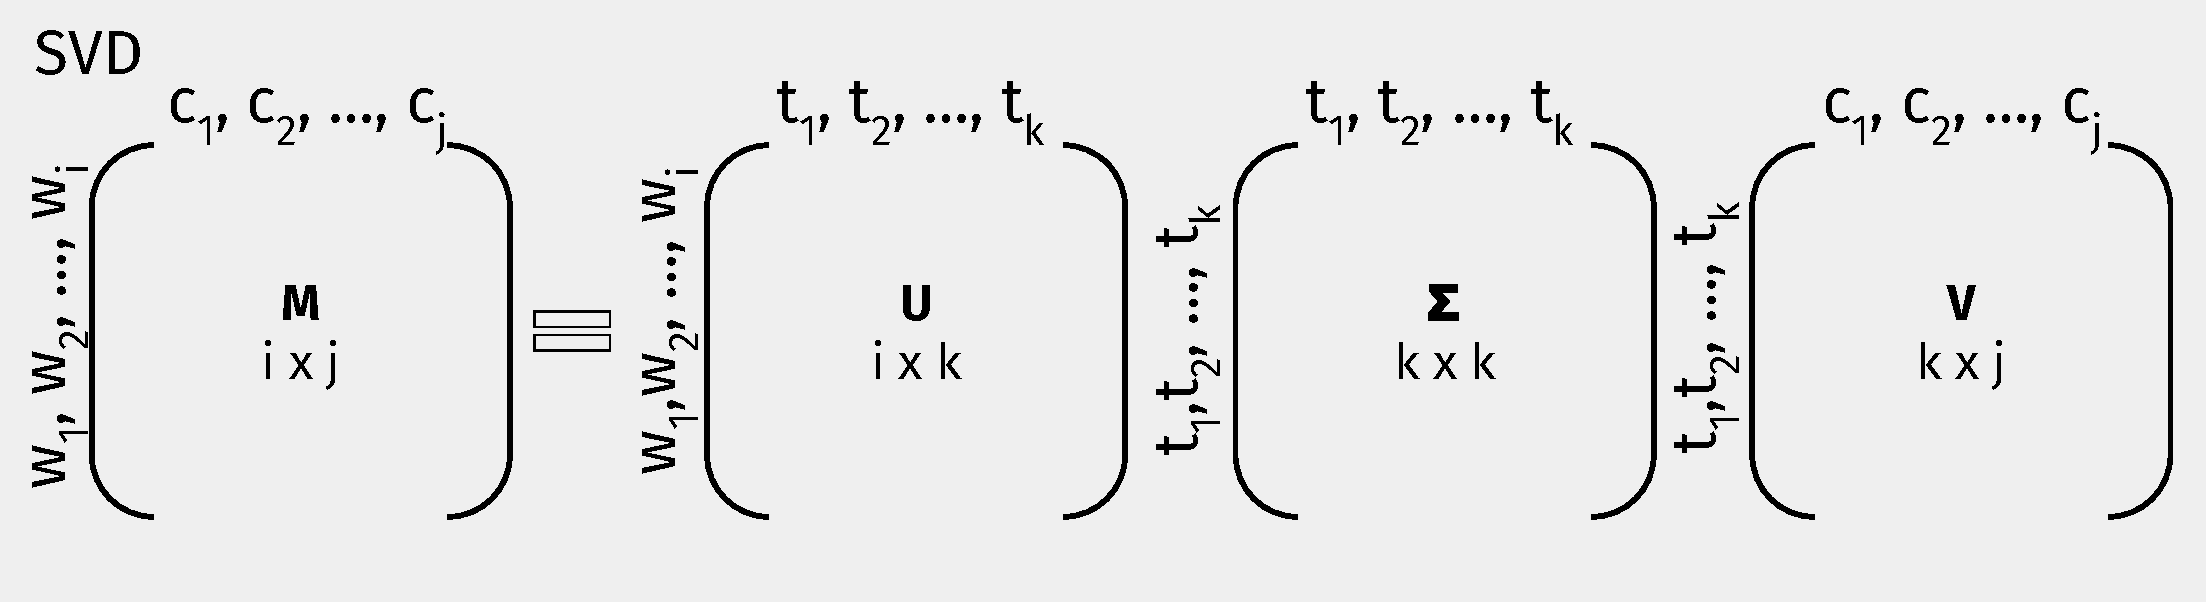
\includegraphics[width=.8\linewidth]{images/Chapitre2/svd.pdf}
\caption{Factorization of the matrix $M$ using SVD. Three matrices are generated: $U$, $\Sigma$, and $V$. $U$ is the one that really interest us, it contains $|W|$ words and $k, k<C$ columns.}
\label{fig:svd}
\end{figure}
%todo HAcer bold the matrix names

Classic examples of implicit representations include Latent Semantic Analysis and Linear Discriminant Analysis, both methods generate a word-document (terms in rows, documents in columns) co-occurrence matrix, weighted by tf-idf. Then, the matrix is reduced into a smaller dimension by means of a Singular Value Decomposition (SVD). SVD keeps the top $k$ singular values that maximize the variance among the features, $k$ being smaller than the original number of dimensions.

Recalling  the  definition of a co-occurrence matrix $M$ (where $f_{ij} \in \mathbb{R}^{W\times C}$), SVD factorizes $M$ into three matrices: two orthogonal matrices $U$ and $V$; and one diagonal, containing ordered eigenvalues $\Sigma$, and $V$, such that $M_{i\times j} = U_{i\times k}\Sigma_{k\times k}V_{k\times j}$, as shown in Figure \ref{fig:svd}. We are interested in matrix $W= U_k\Sigma_k$, as it  contains the words represented by $k$ singular values, and we thus can substitute $M$ with it. In the same fashion, we can obtain the same reduced representation for the contexts by using directly $V_k$. \cite{levy2015improving} found that, empirically, we can even dismiss the eigenvalues matrix $V_k$ in $W$ and obtain better general performance.

% todo cite allison2006another saying that data imporoves results

\begin{figure}
\centering
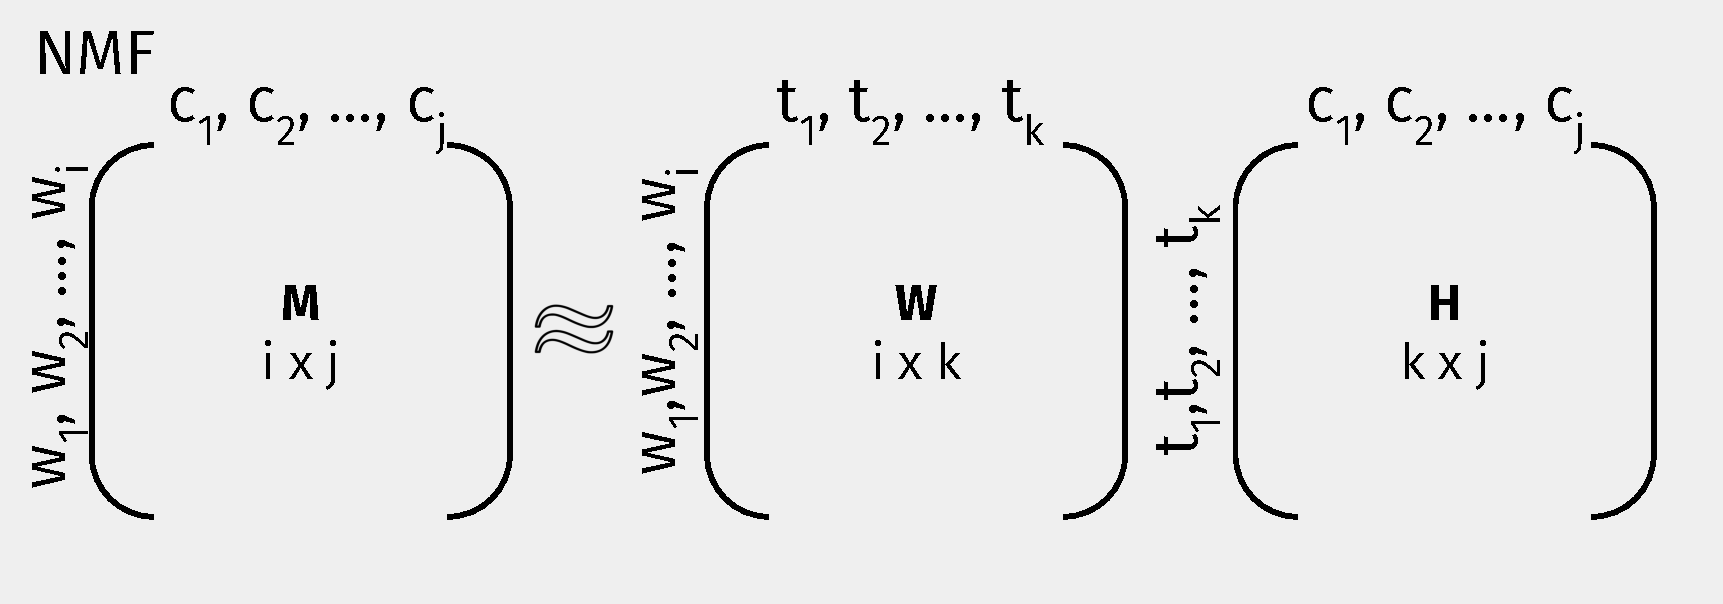
\includegraphics[width=.8\linewidth]{images/Chapitre2/nmf.pdf}
\caption{Factorization of the matrix $M$ using NMF. Two matrices are generated: $W$ and $H$. $W$ contains the words in a $k$ reduced space. $H$ contains the contexts in the reduced space.}
\label{fig:nmf}
\end{figure}

A similar approach, that of the Non-negative Matrix Factorization \cite{lee2001algorithms} (NMF)  is  also used to find latent  dimensions in the co-occurrence matrix. As shown in Figure \ref{fig:nmf}, NMF factorizes $M$ into only two matrices: $M_{i \times j} \approx W_{i\times k} H_{k\times j}$. The first matrix $W$ contains the words represented by a lower dimension $k$. On the other hand, $H$ represents the relation between the contexts and the newly induced dimensions. This procedure solves certain issues with SVD, such as containing only positive values in the factorized matrices, which is more intuitive when dealing with text, i.e., the original matrix is the result of the addition of the factorized values. Also, depending on the implementation, NMF is able to solve the Kullback-Leibler divergence (instead of the Euclidean distance, as SVD) as objective function. This measure is better suited for textual data, for example in the factorization of both lexical and syntactic co-occurrence matrices \cite{VandeCruys2011}.
 

Lastly, the most popular implicit approach nowadays is the use of distributed representations, also known more popularly as word embeddings. The goal is to represent words with a rich dense matrix and relatively few dimensions. These representations are generated from very large bodies of text, creating a regular co-occurrence matrix and calculating, via either a neural network approach \cite{bengio2003neural,Collobert2011,mikolov2013distributed} or a matrix factorization \cite{pennington2014glove,levy2014neural},  a lower dimensional and dense matrix representation. This area is fast developing, with new methods and propositions every few months. Furthermore, the community is not really certain still on which approach is better, either depending exclusively on co-occurrence frequencies and matrix factorization methods, or on sophisticated prediction approaches coupled with neural networks techniques \cite{baroni2014don,levy2015improving}.



\subparagraph{Enriched Explicit Representations}
While implicit representations modify the interpretation of the columns of the co-occurrence matrix so that they are no longer directly interpretable\footnote{Still, the meaning can be inferred to a certain level with the help of the reduced matrices.},  enriched explicit representations modify the meaning of the contexts with the addition of replacement of information to them in order to better cover a larger set of target words and thus reduce the sparsity of the matrix. More importantly, the new contexts are still \textit{natural} concepts in the sense that are still easily interpretable by us humans.




For example, leveraging the large size of the English Wikipedia corpus, the Explicit Semantic Analysis \cite{gabrilovich2007computing} aims to augment text presentation by describing words in terms of Wikipedia concepts. The method yields weighted vectors of Wikipedia concepts that best represent, according to a document ranking, an input text (see Figure \ref{fig:esa}).  The advantage of this representation is that indeed the concepts are human interpretable, not like implicit models, and it covers a very large body of information,  the Wikipedia corpus. As a downside, vectors using this representation tend to be very large, which makes dealing with them may represent a computational challenge.
% What is more, the representations are dependent on the size of the Wikipedia corpus used. 
On the other hand, vectors based on non-English versions may suffer from the reduction of textual data, as the English Wikipedia is considerably larger than most languages.

\begin{figure}
\centering
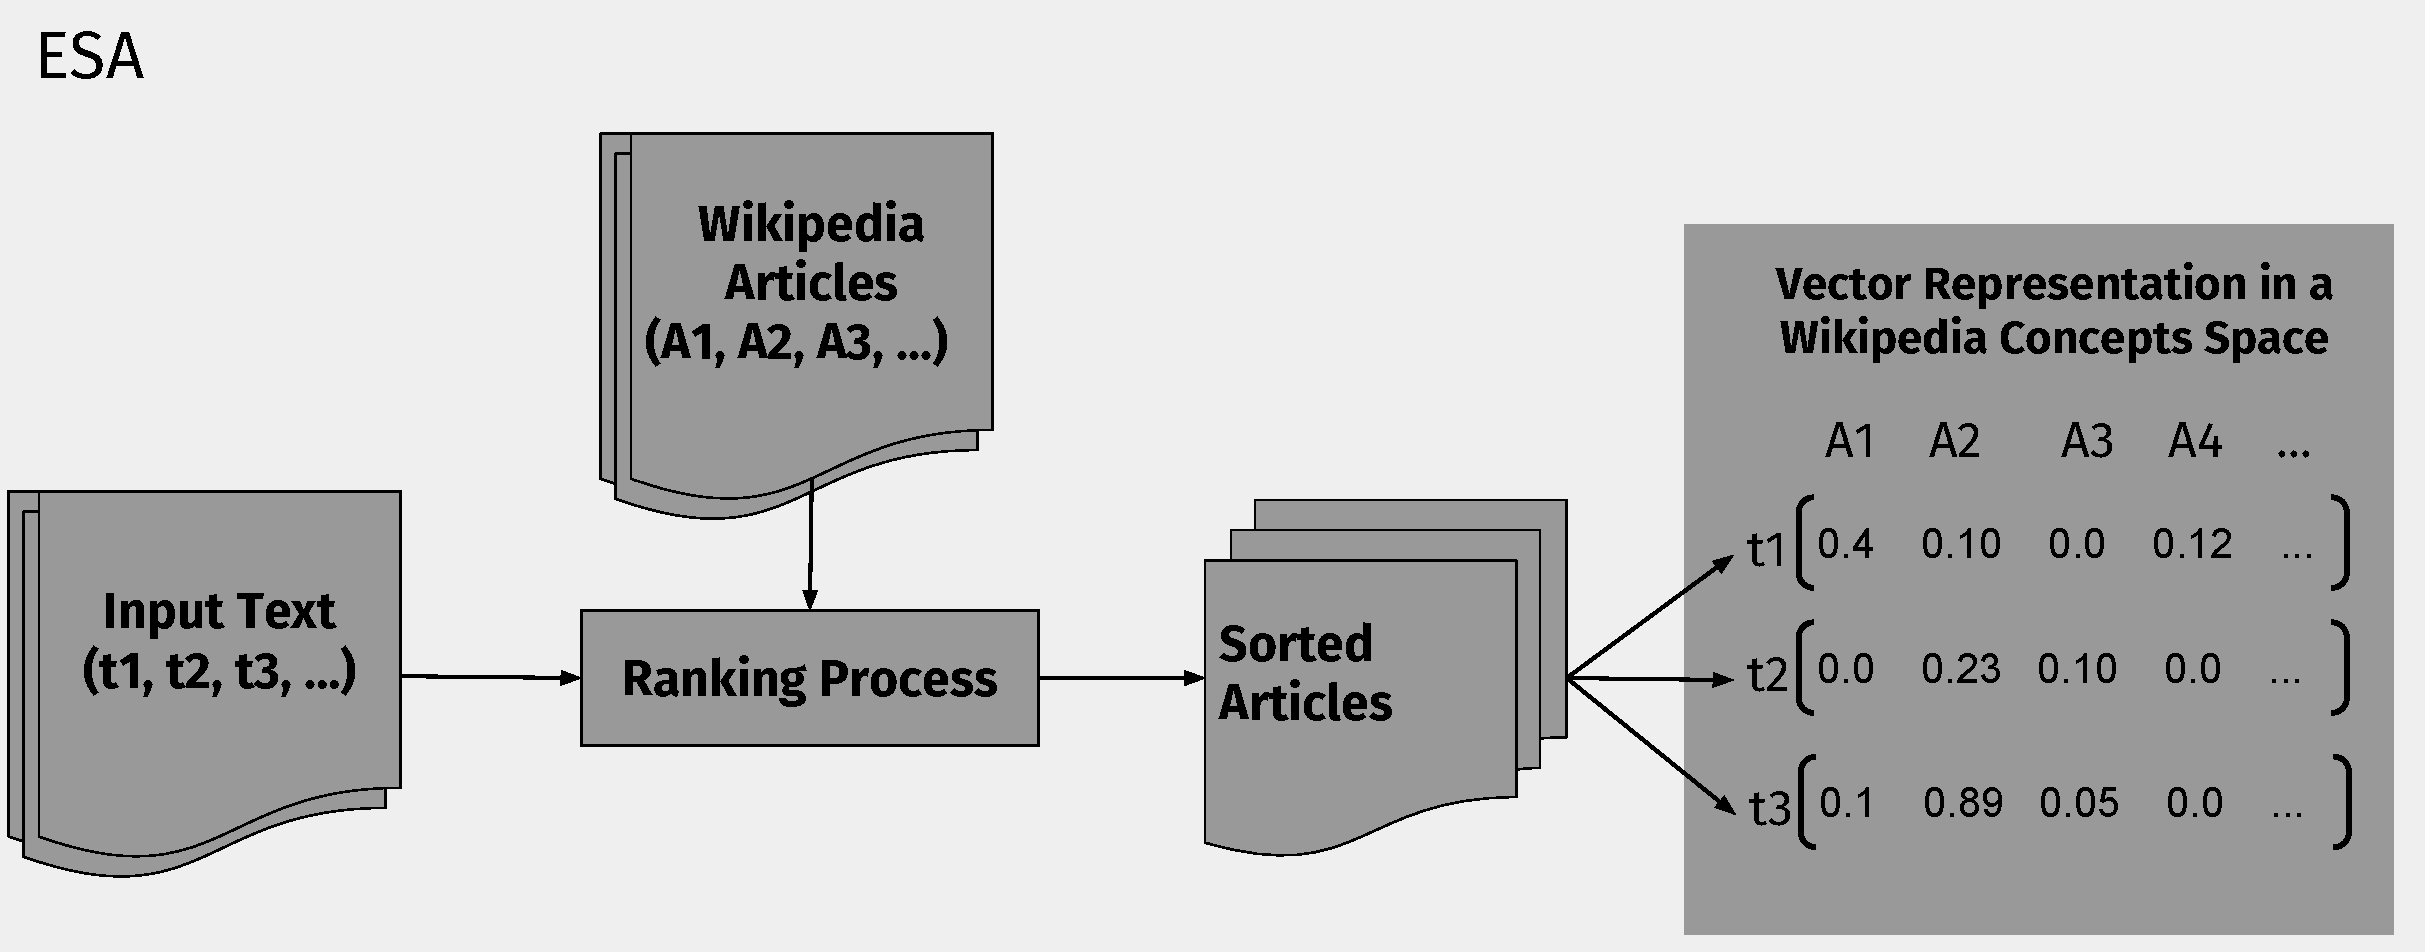
\includegraphics[width=\linewidth]{images/Chapitre2/esa.pdf}
\caption{Block description of the ESA process by \cite{gabrilovich2007computing}. The method ranks Wikipedia articles according to an input document. The document is then described by a weighted vector, where each dimension is a Wikipedia article, or concept.}
\label{fig:esa}
\end{figure}

Fusion techniques are another option to enrich and eventually densify feature spaces.  While not largely applied in the textual analysis domain as in the multimedia information retrieval and phonetics fields \cite{ozkan2010latent,Ah-PineCC15}, they represent a set of simple yet powerful methods to merge information and create more powerful representations. Indeed, these operations are based on the combination of feature spaces  to obtain representations that leverage the complementarity of the original spaces. \cite{bruni2014multimodal} has employed fusion methods to generate enriched multimedia semantic spaces while blending images and text to define the similarity among words. While feature spaces are combined, these techniques do not modify the meaning of the contexts and they remain interpretable. In this thesis, as we described in the introduction of this work, and as we will see later on, we also use these techniques to fight data sparsity by combining linguistic spaces, without resorting to other types of data. Namely,  by leveraging the properties of two distributional representations, both lexical and syntactic co-occurrences, we can get more dense and stronger  word representations. 

%todo random techniques for data spaarsity see \cite{Sahlgreen,Lenci}

\section{Conclusion}

We have introduced four axis that define the work that we carry out in this thesis. Our propositionas are based on the distributional hypothesis: we assume that words that share a common context are related. The relation is determined by the type of context: whether lexical or syntactic properties. If we choose a lexical context, the size of the window (how many words to the right, to the left) should be determined according to the ultimate goal of the NLP task at hand. This window has an effect on the semantic properties of the relatedness among words: the shorter the window, the closer we get to a synonymy similarity, i.e., we may be able to interchange words one for another and keep a coherent phrase. The larger the window, the more topical the relatedness is, i.e., words are related in a broader sense. On the other hand, when using shorter windows we indeed approach to the relatedness provided by syntactic relations \cite{sahlgren2006word}, which relate words that participate in the same syntactic dependency functions, also known as functional similarity \cite{LevyG14}. %Again, this implies that words could be substituted without losing sense within a phrase.

These contexts need to be represented computationally in order to perform some Using co-occurrence matrices, we can keep track of what words are seen with what contexts within a corpus. These counts may then be affected by some weight that determines the relevance of said co-occurrences in terms of uniqueness in terms of the whole set of co-occurrences found. Once these word's vectors are created, we can thus finally calculate a degree of relatedness between them by employing vector similarity metrics, notably the cosine similarity (for real-valued vectors) and Jaccard (binary valued vectors) metrics.

While matrices are the fundamental structure used in computational operations, we can model the links among words intuitively with graph-based structures. Indeed, by modeling text as graphs we gain access to  established graph-theory techniques which helps us elucidate the inner structure of textual data. 	

Whether its vector based or graph based, a textual, explicit, and distributional representation will be sparse. There are too many words in a text and its assured that, while they could occur in other texts, they will not occur in a single text. This becomes an important problem with NLP systems: words are described by only a small set of features.

In the following chapter we describe our two first propositions which address the issue of using heterogeneous information to represent a term and alleviating the data sparsity that comes with such types of textual representations.


%
	

%\section{Graph-based Models}
%
%
%\section{Word Sense Induction and Disambiguation}
%\section{Named Entity Recognition}

%\section{Sequential Classification: Structured Perceptron}
%\section{Clustering: lustering}

%++++++++++++++++++++++++++++++++++++++++++++++++++++++++++++++++++++++++++++++++++++++++++++++++++



